\documentclass[]{elsarticle} %review=doublespace preprint=single 5p=2 column
%%% Begin My package additions %%%%%%%%%%%%%%%%%%%
\usepackage[hyphens]{url}

  \journal{Which journal? Journal of Service Research/Health Services Research/EJOR/IJF} % Sets Journal name


\usepackage{lineno} % add
\providecommand{\tightlist}{%
  \setlength{\itemsep}{0pt}\setlength{\parskip}{0pt}}

\usepackage{graphicx}
%%%%%%%%%%%%%%%% end my additions to header

\usepackage[T1]{fontenc}
\usepackage{lmodern}
\usepackage{amssymb,amsmath}
\usepackage{ifxetex,ifluatex}
\usepackage{fixltx2e} % provides \textsubscript
% use upquote if available, for straight quotes in verbatim environments
\IfFileExists{upquote.sty}{\usepackage{upquote}}{}
\ifnum 0\ifxetex 1\fi\ifluatex 1\fi=0 % if pdftex
  \usepackage[utf8]{inputenc}
\else % if luatex or xelatex
  \usepackage{fontspec}
  \ifxetex
    \usepackage{xltxtra,xunicode}
  \fi
  \defaultfontfeatures{Mapping=tex-text,Scale=MatchLowercase}
  \newcommand{\euro}{€}
\fi
% use microtype if available
\IfFileExists{microtype.sty}{\usepackage{microtype}}{}
\usepackage[top=25mm, left=30mm, right=30mm, bottom=25mm,headsep=10mm, footskip=12mm]{geometry}
\usepackage{natbib}
\bibliographystyle{plainnat}
\usepackage{longtable,booktabs,array}
\usepackage{calc} % for calculating minipage widths
% Correct order of tables after \paragraph or \subparagraph
\usepackage{etoolbox}
\makeatletter
\patchcmd\longtable{\par}{\if@noskipsec\mbox{}\fi\par}{}{}
\makeatother
% Allow footnotes in longtable head/foot
\IfFileExists{footnotehyper.sty}{\usepackage{footnotehyper}}{\usepackage{footnote}}
\makesavenoteenv{longtable}
\ifxetex
  \usepackage[setpagesize=false, % page size defined by xetex
              unicode=false, % unicode breaks when used with xetex
              xetex]{hyperref}
\else
  \usepackage[unicode=true]{hyperref}
\fi
\hypersetup{breaklinks=true,
            bookmarks=true,
            pdfauthor={},
            pdftitle={Forecasting short-term hourly Emergency Departement arrivals},
            colorlinks=false,
            urlcolor=blue,
            linkcolor=magenta,
            pdfborder={0 0 0}}
\urlstyle{same}  % don't use monospace font for urls

\setcounter{secnumdepth}{5}
% Pandoc toggle for numbering sections (defaults to be off)

% Pandoc citation processing

% Pandoc header
\usepackage{adjustbox, float,lscape, bm,amsmath}
\usepackage{booktabs}
\usepackage{longtable}
\usepackage{array}
\usepackage{multirow}
\usepackage{wrapfig}
\usepackage{float}
\usepackage{colortbl}
\usepackage{pdflscape}
\usepackage{tabu}
\usepackage{threeparttable}
\usepackage{threeparttablex}
\usepackage[normalem]{ulem}
\usepackage{makecell}
\usepackage{xcolor}



\begin{document}
\begin{frontmatter}

  \title{Forecasting short-term hourly Emergency Departement arrivals}
    \author[University1]{Bahmna Rostami Tabar\corref{1}}
   \ead{email1@example.com} 
    \author[School of Mathematics and Statistics, University of Glasgow, UK]{Jethro Browell\corref{2}}
   \ead{jethro.browell@glasgow.ac.uk} 
    \author[Centre for Marketing Analytics and Forecasting, Lancaster University, UK]{Ivan Svetunkov\corref{2}}
   \ead{i.svetunkov@lancaster.ac.uk} 
      \address[University1]{Cardiff business school, 3 Colum Drive, CF10 3EU, Cardiff}
    \address[University2]{adress2}
    \address[University3]{adress3}
      \cortext[1]{Corresponding Author}
    \cortext[2]{Equal contribution}
  
  \begin{abstract}
  The Objective of this work would be to propose a new methodology to forecast short-term hourly forecasting for urgent and emergency care.
  \end{abstract}
  
 \end{frontmatter}

\hypertarget{introduction}{%
\section{Introduction}\label{introduction}}

Forecasting Emergency Department (ED) arrivals is critical for informing staffing and scheduling decisions to meet the needs of patients. An accurate ED demand forecasts contribute to a better decision making process regarding the resources allocation and staffing. This is one of the best ways to optimize resources utilisation and minimise related costs. State of the art practice to optimise personnel scheduling follows the general approach originally presented by \citet{vile2016time}, which recommends that the following steps be taken to roster employees: (i) forecast demand; (ii) convert demand forecasts into staffing requirements; (iii) schedule shifts optimally; and (iv) assign employees to shifts. An accurate demand forecasting is crucial in ED services to depict various courses of action that can result in massive savings in terms of patient lives. Inability to match the staff with the demand might result in patients overcrowding the system which is a serious problem that causes challenges for the patient flow \citep{derlet2002overcrowding}. Also, it is related with increasing length of stay \citep{muhammet2015forecasting}, low patient satisfaction, unexpected return visits to services, increased health care costs, inaccuracy in electronic medical records and other \citep{rostami2020anticipating}.

An accurate forecasting of arrivals by hour of the day enables planners to match staff to meet anticipated patients, reconfigure units and redeploy staff. This has many advantages for both patients, staff and the quality of provided services. Hourly forecasts are required to inform the short-term operational planning for the current and the upcoming shifts of the day. This involves the short-term decision making related to the execution of the delivery process in ED.
The combination of an hourly forecast demand, current staff being occupied, resource availability and waiting times at ED, provide information on the state of the unscheduled care system across the service. Having this full picture enables the delivery managers to focus on the areas that require intervention to enable the most effective delivery of the service to the patients. However, in comparison with lower frequency time series forecasting such as monthly, quarterly and yearly, hourly forecasts are challenging because the noise caused by random variation may overshadow any pattern in the time series. Hourly time series generally exhibit multiple seasonal cycles of different lengths such as hourly, daily, weekly and yearly. They may also express nonstationarity and their profile may change over time. Therefore, an appropriate forecasting model should take these features into account, to accurately predict hourly demand admissions.

There are few studies that look at forecasting hourly arrivals in ED and other hospital services using historical time series data and/or predictors such as patient characteristics , climate factors , holidays. These studies use multiple approaches including Exponential Smoothing \citep{SvetunkovAdam}, Autoregressive Integrated Moving Average (ARIMA) \citep{hyndman2021forecasting}, Autoregressive Conditional Heteroskedasticity (ARCH) \citep{bollerslev1994arch}, Vector Autoregressive model \citep{lutkepohl2013vector}, TBATS \citep{de2011forecasting} and Artificial Neural Networks \citep{hyndman2021forecasting}. There are few limitations in these studies. They only generate the estimated future arrivals as a point forecast (a single number), which does not acknowledge any uncertainty around the number of arrivals. However, reporting uncertainty is critical because the consequences of imperfect staffing are asymmetric. This asymmetry arises because it is preferable to incur a small opportunity cost associated under utilised staff rather than lower service levels if staff levels are insufficient. This is where producing probabilistic forecasts could be beneficial in staffing. The lack of probabilistic forecast is one of the main bottlenecks in the deployment of generated forecasts in the staffing and planning tools in practice. Probabilistic forecasts are necessary to make decisions that balance the cost associated with under and over staffing. In this paper, in adition to generating point forecast, we also produce and evaluate the forecast distribution of hourly ED arrivals, using several forecasting models, which could be used as a risk management tool for planners and decision makers. Moreover, datasets used in some of these studies are relatively small, short length (e.g.~time period of 1 year), which make it challenging to report the forecast accuracy using robust approaches such as time series cross validation and such results might not be reliable. Additionally, most of forecasting methods used in these publications does not consider the multiple seaonality natutre of hourly ED arrivals. Moreover, all previous publicationscovered in this paper fails reproducibility principles.

In this paper, we aim at filling several gaps, and our contributions to the literature are summarised as follows:

\begin{enumerate}
\def\labelenumi{\arabic{enumi}.}
\item
  We use the family of Generalised Additive Models to forecast short-term hourly hospital admission using that accounts for i) \ldots, ii) \ldots{} iii) , \ldots{} iv) (Jethro to complete)
\item
  We apply advanced dynamic model based on iETS \citep{Svetunkov2019a} and ETSX models with a modification for multiple frequencies;
\item
  We produce probabilistic forecasts, in addition to the point ones, quantifying the uncertainty in future hospital admission;
\item
  We compare the accuracy of our models with the one from the well established benchmarks, such as Prophet, TBATS, Poisson Regression, and exponential smoothing state space model (ETS);
\item
  We provide data and code enabling reproduction and refinement of the proposed approach and benchmarks. The proposed approach could also be generalized to forecast hourly requirements in other services such as the number of incidents or call volumes in clinical desk services.
\end{enumerate}

The rest of the paper is organised as following: section \ref{lit} provides a brief overview of hourly ED arrival forecasting in healthcare. Section \ref{model} starts with \ldots{}

\hypertarget{lit}{%
\section{Research background: hourly ED forecasting}\label{lit}}

There are many studies that employ models to forecast the admission and arrivals in Emergency Department. The time granularity considered by these studies spans from hourly to yearly. However, given the focus of the paper, we only discuss the hourly ED forecasting. Table \ref{tab:summarylit} summarize the relevant papers.

\begin{landscape}\begin{table}[!h]

\caption{\label{tab:summarylit}Summary of studies in forecasting hourly arrivals in Emergency Department}
\centering
\resizebox{\linewidth}{!}{
\fontsize{11}{13}\selectfont
\begin{tabular}[t]{lr>{\raggedright\arraybackslash}p{6em}>{\raggedright\arraybackslash}p{4em}l>{\raggedright\arraybackslash}p{15em}>{\raggedright\arraybackslash}p{4em}ll}
\toprule
Author & Year & Variable & Horizon & Length & Method & Metric & Probabilistic & Multiple seasonality\\
\midrule
Choudhury and Urena & 2020 & ED arrivals & 1h to 24h & 4 & ARIMA; Holt-winters; TBATS; ANN & RMSE, ME & No & Yes\\
Asheim et al. & 2019 & ED arrivals & 3h & 5 & Poisson regression & MAPE & No & No\\
Hertzum & 2017 & ED arrivals & 1,2,4,8,24 hours & 3 & linear regression; SARIMA; Naïve & MAE, MAPE, 
MASE & No & No\\
Kim et al. & 2014 & Hospital admission & 4h, 24h & 3 & Linear regression; Exponential smoothing; ARIMA; GARCH; VAR & MAPE & No & No\\
Cote et al. & 2013 & ED arrivals & 24h & 2 & Fourier regression & R\textasciicircum{}2,  Standard Error & No & No\\
Chase et al. & 2012 & ED CUR & 30m
1h, 2h, 4h, 8h, 12h & 1 & Binary regression & NA & No & No\\
Schweigler et al. & 2009 & Bed occupancy & 4h, 12h & 4 & Hourly historical average; SARIMA; Sinusoidal model with autocorrelated error & RMSE & No & No\\
Jones et al. & 2009 & ED census & 24h & 2 & VAR;  Holt winters & MAE & No & No\\
McCarthy & 2008 & ED arrivals & 24h & 2 years & Poisson log-linear regression model & 95\% CI & No & Yes\\
Channouf et al. & 2007 & Ambulance admission & 1h, 3h, 6h, 12h, 13h, 14h, 17h, 23h, 24h & 2 & Regression & RMSE & No & No\\
Morzuch and Allen & 2006 & ED arrivals & 168h & 3 & Regression; ARIMA; Exponential smoothing & RMSE & No & No\\
\bottomrule
\end{tabular}}
\end{table}
\end{landscape}

Linear regression, ARIMA, and Naïve were used by \citet{hertzum2017forecasting} to investigate whether accurate hourly accident and emergency department patient arrivals and occupancy forecasts can be generated using calendar variables. Naïve method was there for the purpose of comparison. \citet{hertzum2017forecasting} study shows that patient arrivals variation is larger across the hours of the day than across the days of the week and the months of the year. In terms of hour of the day, patient arrivals peaked around noon. For days of the week, Monday is the busiest day while weekends are the quietest ones. July-August are the months with the highest numbers of patient arrivals, while January and February are the months with the lowest numbers. According to \citet{hertzum2017forecasting}, the regression and ARIMA models performed similarly in modelling patient arrivals, while ARIMA outperformed regression models in modelling accident and emergency department occupancy. However, after all, the models of occupancy were less accurate than those of arrivals. \citet{hertzum2017forecasting} mentioned that ARIMA was among the most accurate models in terms of forecasting accident and emergency department visits.

\citet{choudhury2020forecasting} used ARIMA, Holt-Winters, TBATS, and neutral network methods to forecast hourly accident and emergency department arrivals. ARIMA model was selected as the best fit model. Authors claimed that ARIMA has provided high and acceptable hourly ED forecasting accuracy, even outperforming TBATS.

\citet{morzuch2006forecasting} used the Unobserved Components Model (UCM), in which each component of the time series is separately modeled as stochastic. Double-seasonal exponential smoothing and standard Holt-Winters were used to forecast ED arrival for an horizon of 168 hours. The hourly data collected from an ED in Pennsylvania showed no trend, and two seasonal cycles: a within-day and a within-week seasonal cycles. The double seasonal model recorded lower RMSEs for all the 168-hour horizons, which was expected due to the strong hourly seasonality of the time series.

\citet{mccarthy2008challenge} employed a Poisson log-linear regression model, including independent variables such as temporal factors (e.g., hour-of-day, day- of-week, type-of-day, season, and calendar year), patient characteristics (i.e., age, gender, insurance status, triage level, mode of arrival, and ambulance diversion status) and climatic factors (i.e., temperature and precipitation) to forecast patient demand for ED services. Hourly data of ED arrivals in the 1-year study period was deployed to forecast from 1 hour to 24 hours into the future. The authors presented the prediction intervals with \(50\%\) and \(90\%\) confidence levels for the number of hourly arrivals under the Poisson assumption. They showed that the most important predictor was hour of the day and AR(1).

\citet{schweigler2009forecasting} conducted an investigation on whether time series methods could accurately generate short-term forecasts of ED bed occupancy. A year-long dataset of hourly ED bed occupancy was collected from three facilities. For each facility, the authors implemented an hourly historical average model, SARIMA model and sinusoidal model with autocorrelated error. The historical average model was based on the mean occupancy for each site, for each hour of the day; while the sinusoidal model was based on 4 parameters: an AR term, a sine coefficient, a cosine coefficient and an intercept. They evaluated the forecast accuracy of four and twelve hours forecast horizon using RMSE and they found that both SARIMA and the sinusoidal models outperformed the historical average (for example, at site 2, the two models improved by \(33\%\) the 12-hour forecasts generated by historical average).

\citet{kim2014predicting} compared different univariate and multivariate time series forecasting techniques to forecast patient volume for a Hospital Medicine programme. The study evaluated linear regression, exponential smoothing, ARIMA, SARIMA, GARCH (generalized autoregressive conditional heteroskedasticity method) and vector autoregressive (VAR) models to forecast for 4 hours and 24 hours ahead. They used MAPE to report the forecast accuracy. ARIMA model outperformed all the other models.

\citet{asheim2019real} developed a Poisson time-series regression model with continuous day-of-week and week-of-year effects to implement a real-time system that could forecast ED arrivals on 1, 2, 3 hours ahead. Measuring the accuracy using the MAPE, \citet{asheim2019real} noticed that great improvement happened when time of notification was incorporated into the model, especially in one-hour horizon.

According to the studies mentioned above, it can be said that they have shown complications in forecasting hourly patient accident and emergency department visits and the application of forecasting hourly patients visits is not well established. Some of the studies claimed that the accuracy of forecasting models on hourly accident and emergency department data forecasting model is low compared to the higher forecasting intervals, like daily \citep{boyle2012predicting, hertzum2017forecasting}. However, some studies mentioned that the accuracy of ED hourly forecast is at the acceptable level \citep{choudhury2020forecasting, mccarthy2008challenge, schweigler2009forecasting}.

There are few limitations in the literature which encourage us to undertake this research and examine different forecasting approaches. These limitations are summarised as follows:

\begin{enumerate}
\def\labelenumi{(\roman{enumi})}
\tightlist
\item
  Current approaches to forecast hourly ED arrivals do not fully consider the feature of data such as multiple seasonal cycles and changing profile over time;
\item
  Almost all research studies produce point forecasts and consequently report only point forecast accuracy. There is a lack of studies presenting probabilistic forecasts of hourly ED arrivals that better represent uncertainty of future admissions, providing a holistic picture of future demand for a planner;
\item
  most studies are not reproducible, as it is almost impossible to reapply the approaches without the helpf of the authors of those papers;
\item
  studies are limited in terms of the length of historical data used for training purposes and forecast performance evaluation and
\item
  some studies in this area lack a rigorous experimental design, i.e.~there is no benchmark method or forecast accuracy is not reported.
\end{enumerate}

\hypertarget{data}{%
\section{Preliminary analysis}\label{data}}

Data used in this study comprises counts of patients' arrival times at one of the largest ED units in the UK between April 2014 and February 2019, extracted from the ED administrative database of the hospital. We aggregated the patients' arrival times to obtain hourly arrivals, which is used for empirical evaluation in this study.

Figure \ref{fig:hourly-plot-ridge} illustrates the distribution of arrivals for each hour of the day and the day of the week. Although the data is noisy, it reveals some systematic patterns.

\begin{figure}[H]

{\centering 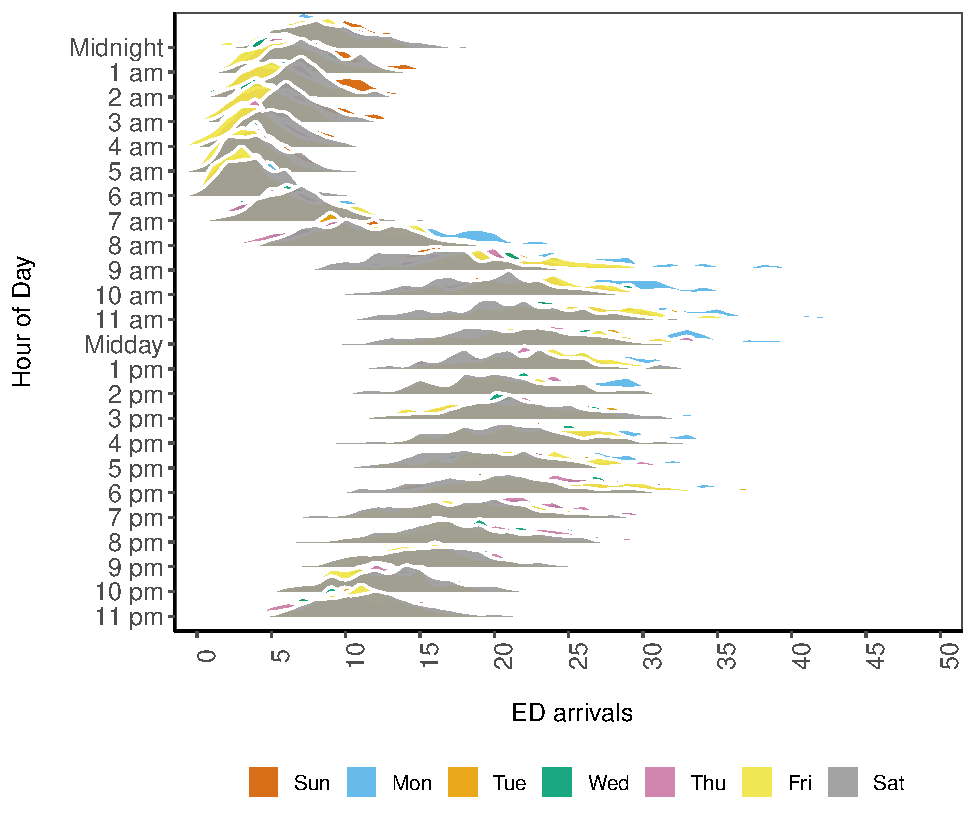
\includegraphics{paper_files/figure-latex/hourly-plot-ridge-1} 

}

\caption{Distrubution of admission per hour and day of the week}\label{fig:hourly-plot-ridge}
\end{figure}

It is clear that the number of arrivals has a sub-daily structure, similar to the one summarised by \citet{hertzum2017forecasting}. The ED arrivals decrease between mid-night and early morning and then increase until the evening, decreasing after that again. It is also clear that ED service gets systematically more visits on Mondays between 8 a.m. and 5 p.m. Moreover, The number of arrivals around mid-night is slightly higher for Saturday and Sunday.

Figure \ref{fig:hourly-plot-ridge} also highlights that there are many ouliers for almost every hour of the day that may affect the accuracy of forecasting methods. Some of these outliers might be related to holidays and special events. It is also clear that arrivals are less volatile between mid-night and early morning.

\begin{figure}[H]

{\centering 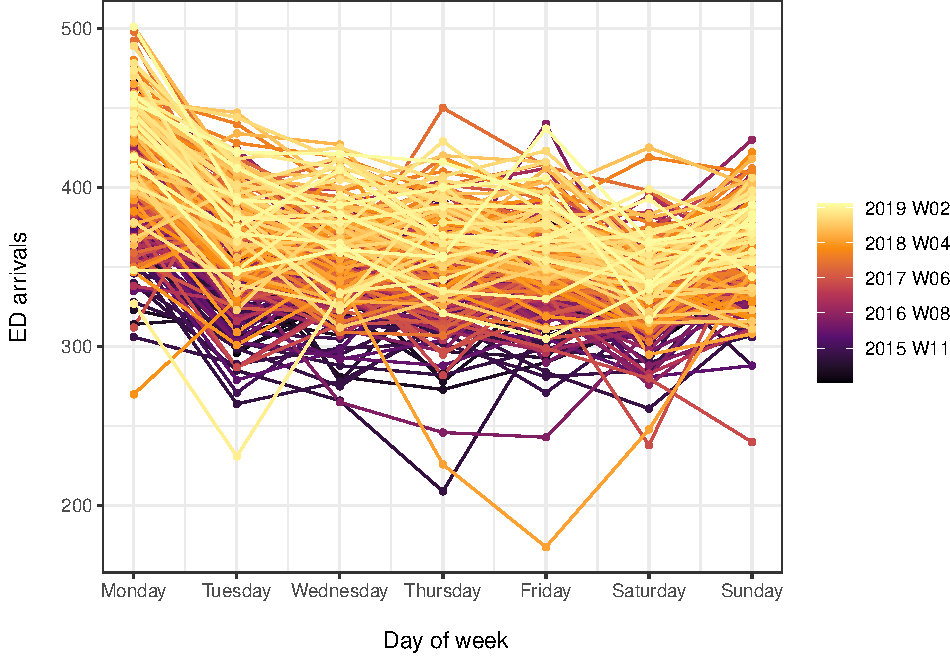
\includegraphics[width=0.7\linewidth]{paper_files/figure-latex/seasonplot-dofw-1} 

}

\caption{Seasonal plot: day of week arrivals}\label{fig:seasonplot-dofw}
\end{figure}

\textbf{IS: We need to plot day of week and week of year seasonalplots here and discuss. This will show multiple seasonality nature of the data.}

\begin{figure}[H]

{\centering 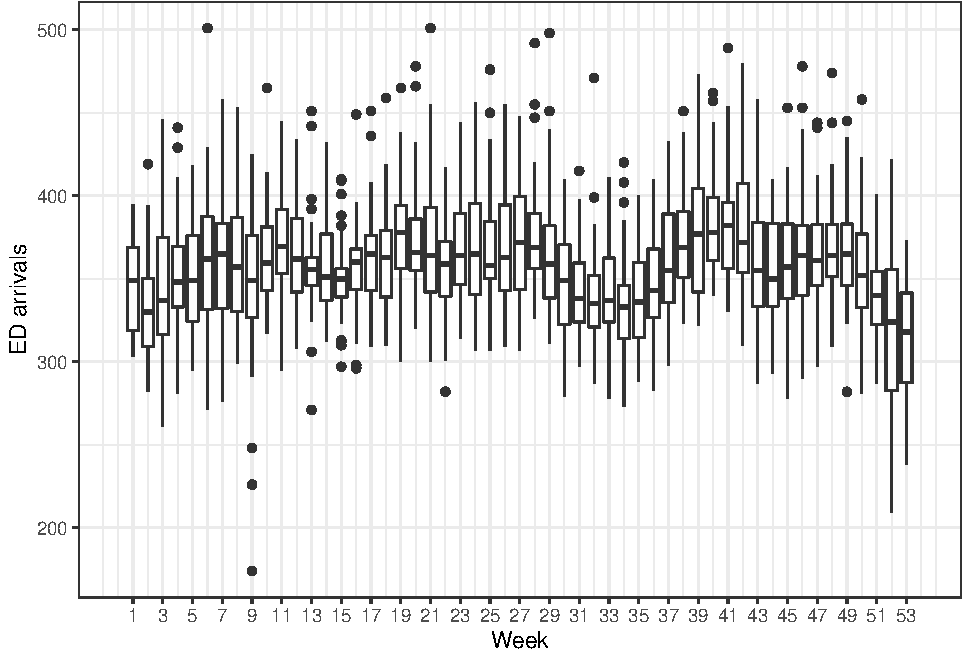
\includegraphics[width=0.7\linewidth]{paper_files/figure-latex/seasonplot-weekofyear-1} 

}

\caption{Week of year arrivals}\label{fig:seasonplot-weekofyear}
\end{figure}

\begin{figure}[H]

{\centering 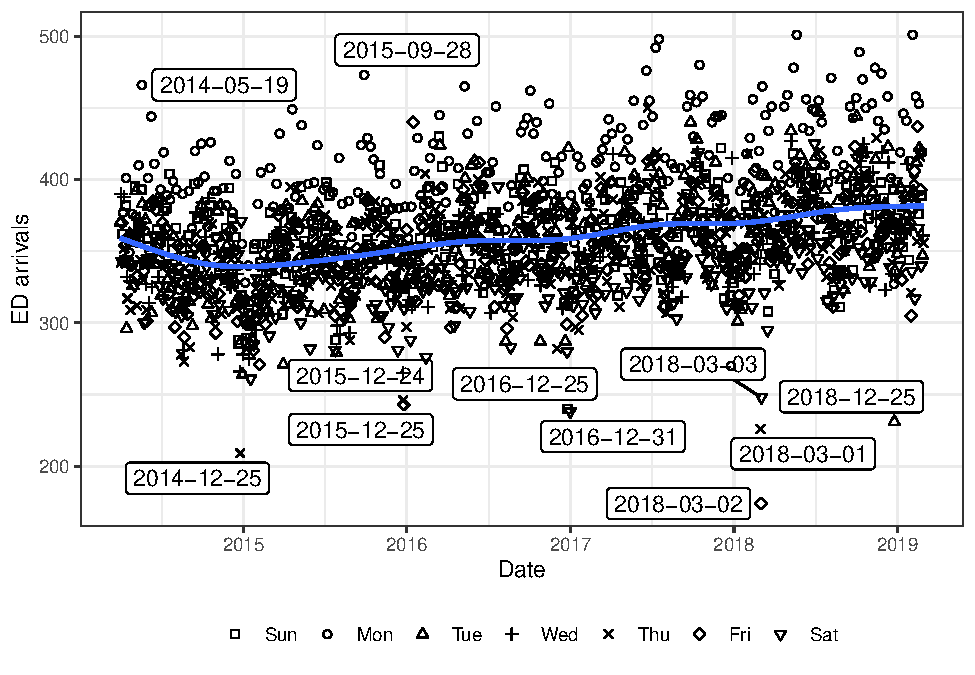
\includegraphics[width=0.7\linewidth]{paper_files/figure-latex/date-plot-1} 

}

\caption{Daily arrivals}\label{fig:date-plot}
\end{figure}

Based on this simple analysis, we should consider model that could take the following into account:

\begin{itemize}
\tightlist
\item
  Hour of day, day of week, and week of year seasonal patterns,
\item
  Calendar events, such as holidays,
\item
  Lags of calendar events to accommodate the potential changes in demand the next day after a holiday,
\item
  Potentially changing level of data,
\item
  Other events, such as football matches in the area.
\end{itemize}

We propose several forecasting models that account for the structures outlined above.

\hypertarget{model}{%
\section{Model building}\label{model}}

\hypertarget{climatology}{%
\subsection{Naive/Climatology}\label{climatology}}

We start with one of the simplest forecasting approaches used in practice - the one that assumes that in the next few hours, everything will be the same as in the similar hours of a similar day in the past. This is called ``Naïve''. In our case, given that we need a distribution of values, we will use a modified approach, used in climatology, where the empirical distribution of demand is used to forecast the future demand distribution. \textbf{We need references here\ldots{}}

\hypertarget{multiple-regression}{%
\subsection{Multiple Regression}\label{multiple-regression}}

Regression is one of the most popular forecasting methods that uses explanatory variables to predict a variable of interest (in our case, the ED arrivals). The classical linear regression model is formulated as:

\begin{equation}
  {y}_t = \mathbf{x}_t' \boldsymbol{\beta} + \epsilon_t ,
\label{eq:linearRegression}
\end{equation}

where \(\mathbf{x}_t\) is the vector of explanatory variables, \(\boldsymbol{\beta}\) is the vector of parameters, \(\epsilon_t\) is the error term, which is typically assumed to follow Normal distribution with zero mean and a fixed variance, and \(t\) is the time index. However, in the context of healthcare and ED arrivals, the assumption of Normality is unrealistic, because the number of admitted patients is integer and non-negative. So the linear regression model should be substituted by some other model. One of the models that is frequently used in practice is the Poisson regression \citep[see for example,][]{mccarthy2008challenge}, which can be summarised as:

\begin{equation}
  \begin{aligned}
    & {y}_t \sim \mathrm{Poisson} \left( \lambda_t \right) \\
    & \log \lambda_t = \mathbf{x}_t' \boldsymbol{\beta}
  \end{aligned}
\label{eq:PoissonRegression}
\end{equation}

The logarithm in \eqref{eq:PoissonRegression} is needed in order to make sure that the parameter of Poisson distribution is always positive. This model can be estimated via maximisation of the likelihood function based on Poisson mass function {[}reference needed{]}. When it comes to selecting explanatory variables for the model, there is no single correct answer, and the decision needs to be done for each specific case. In our experiment, we will only include dummy variables, capturing a variety of calendar events:

\begin{enumerate}
\def\labelenumi{\arabic{enumi}.}
\tightlist
\item
  Hour of day,
\item
  Day of week,
\item
  Week of year,
\item
  Holidays (such as Christmas, New Year etc),
\item
  24 hours lags of holidays.
\end{enumerate}

The variables (1) - (3) allow modelling the seasonal patterns on the appropriate level of detail throughout the year, while (4) covers the changes in admittance due to calendar events. Finally (5) is needed in order to capture the potential phenomenon of change in admittance after the holiday (e.g.~people might try not to go to hospital on Christmas eve and thus will go the next day). This model assumes that all these effects are deterministic and do not change over time, but the exponentiation in \eqref{eq:PoissonRegression} introduces an interaction effect between dummy variables, so that the 3pm on Monday in January will be different from 3pm on Monday in July, although the parameters for hour of day and day of week are fixed and do not change over time. We use \texttt{alm()} function from \texttt{greybox} package \citep{Svetunkov2021Greybox} for R \citep{RTeam2021} for the experiments and denote this model as ``Poisson Regression''.

\hypertarget{ets---exponential-smoothing-model}{%
\subsection{ETS - Exponential Smoothing model}\label{ets---exponential-smoothing-model}}

\citet{Hyndman2008b} developed a state space approach for exponential smoothing models, according to which the model can have a set of components, including different types of Error, Trend and Seasonal component (thus \emph{ETS}). Given the popularity of ETS model in forecasting community, we decided to include the basic ETS(A,N,A) model with the seasonal component with frequency 24 (hour of day) as a benchmark. This was done using \texttt{adam()} function from \texttt{smooth} package \citep{Svetunkov2021Smooth} for R and denote as \emph{ETS}. This model does not capture the day of week or week of year effects, does not include explanatory variables, but its seasonal component and level change over time. This model is included as a benchmark, only to see how the other models perform in comparison with it.

\hypertarget{prophet}{%
\subsection{Prophet}\label{prophet}}

Prophet is a forecasting procedure created by Facebook \citep{taylor2018forecasting} that accounts for multiple seasonality, piecewise trend and holiday effects. Prophet is robust to missing data and shifts in the trend, and typically handles outliers well. Prophet works well on daily data seen in Facebook. It is robust and automated, making it easy to learn for beginners. The implementation may be less flexible than other methods. The model itself relies on Multiple Source of Error state space model, originally proposed by \citet{Kalman1960}. The model is incorporated using corresponding implementation of the Fable package in R. We use the \texttt{prophet()} function from the \texttt{fable} package \citep{fable2020}. Note that the input data is assigned with an hourly and daily seasonality.

\hypertarget{tbats}{%
\subsection{TBATS}\label{tbats}}

\citet{de2011forecasting} proposed a model to deal with time series exhibiting multiple complex seasonalities called ``TBATS''. It includes a Box-Cox Transformation, ARMA model for residuals and a trigonometric expression of seasonal terms. The latter one not only gives the model more flexibility to deal with fractional seasonality but also reduces the parameters of model when the frequencies of seasonalities are high. We fit a TBATS model using the \texttt{tbats()} function from the \texttt{forecast} package in R \citep{forecastpackage2020}.

\hypertarget{adam-multiple-seasonal-ietsx}{%
\subsection{ADAM: multiple seasonal iETSX}\label{adam-multiple-seasonal-ietsx}}

\citet{SvetunkovAdam2021} proposed a framework for dynamic models called \textbf{ADAM} - Augmented Dynamic Adaptive Model. This framework encompasses ARIMA \citep{Box1976}, ETS \citep{Hyndman2008b} and regression, supporting multiple frequencies, non-normal distributions and intermittent demand \citep{Svetunkov2019a}. Based on this framework, we use Gamma distribution for ETS(M,N,M) model with frequencies 24 (hour of day) and 168 (hour of week), adding dummy variables for week of year, holidays and lagged holidays. This way we update the hour of day and day of week seasonal indices, keeping the week of year one fixed, thus reducing the number of estimated parameters. Given that the data exhibits randomly occurring zeroes, we use the direct probability model developed by \citet{Svetunkov2019a} to treat those values. This model can be formulated as a set of the following equations:

\begin{equation}
    \begin{aligned}
      & y_t = o_t z_t \\
        & \log z_t = \log l_{t-1} + \log s_{1,t-24} + \log s_{2,t-168} + \mathbf{x}_t' \boldsymbol{\beta} + \log \left(1 + \epsilon_{t} \right) \\
        & \log l_{t} = \log l_{t-1} + \log( 1  + \alpha \epsilon_{t}) \\ 
        & \log s_{1,t} = \log s_{1,t-m} + \log( 1  + \gamma_1 \epsilon_{t}) \\
        & \log s_{2,t} = \log s_{2,t-m} + \log( 1  + \gamma_2 \epsilon_{t}) \\
        & o_t \sim \text{Bernoulli} \left(\mu_{a,t} \right) \\
        & a_t = l_{a,t-1} \left(1 + \epsilon_{a,t} \right) \\
        & l_{a,t} = l_{a,t-1}( 1  + \alpha_{a} \epsilon_{a,t}) \\
        & \mu_{a,t} = \min(l_{a,t-1}, 1)
    \end{aligned} ,
    \label{eq:ADAMModel}
\end{equation}
where \(\alpha\), \(\beta\), \(\gamma_1\), \(\gamma_2\) and \(\alpha_a\) are the smoothing parameters, defining how adaptive the components of the model should be, \(l_t\) is the level component for the demand sizes, \(s_{1,t}\) and \(s_{2,t}\) are the seasonal components, \(\boldsymbol{\beta}\) is the vector of parameters for the explanatory variables, \(o_t\) is the binary variable, which is equal to one, when demand occurs and to zero otherwise, \(l_{a,t-1}\) is the level component for the occurrence part of the model, and \(\left(1+\epsilon_t \right) \sim \Gamma(s^{-1}, s)\), where \(s=\frac{1}{T} \sum_{t=1}^{T} e_{t}^2\) is the scale of the distribution. Finally, \(a_t\) is an unobservable series, underlying the occurrence part of the model and \((1 + \epsilon_{a,t})\) is an unobservable error term for \(a_t\). \citet{Svetunkov2019a} discuss how to estimate such model. We expect this model to perform on par with the Poisson regression, potentially outperforming it in some instances, due to the dynamic parts of the model (level and seasonal components). Although the data is integer-valued, we expect that Gamma distribution will be a good approximation for it. If integer-valued quantiles are needed, then rounding up can be done for them (see @ref(quantiles\_ceiling) for the explanation). This model is implemented in \texttt{adam()} function from \texttt{smooth} package \citep{Svetunkov2021Smooth} for R and is denoted in our experiment as ``ADAM-iETSX''.

\hypertarget{gamlss}{%
\subsection{GAMLSS}\label{gamlss}}

If we assume that our predictive distribution follows a given parametric distribution, the forecasting task becomes ones of predicting the future values of that distribution's parameters. Generalised Additive Models for Location, Scale and Shape (GAMLSS) are distributional regression models where the parameters may be modelled as additive functions of explanatory variables. This provides a powerful and flexible framework for probabilistic forecasting, provided that a suitable distribution and additive structures can be found. In practice, this means experimenting with various distributions and evaluating their suitability using available training data.

Let \(F_t(y_t)\) be a predictive cumulative probability distribution of \(y_t\). In a distributional regression context, \(F_t(y_t)\) is modelled via a parametric model, \(F(y_t|\bm \theta_t)\), where \(\bm \theta_t\) is an \(m\)-dimensional vector of parameters. In a GAMLSS framework of \citet{Rigby2005} the elements \(j=1,...,m\) of \(\bm \theta_t\) are modelled via:

\begin{equation}
    g_j(\theta_{j,t})=\mathbf{A}_{j,t} \bm{\beta}_j + \sum_{i} f_{j,i}({\bm x}^{S_{j,i}}_t), \;\;\; \text{for} \;\;\; j = 1, \dots, m,
    \label{eq:basicGAM}
\end{equation}

where \(g_j\) is a monotonic \texttt{link} function, \(\mathbf{A}_{j,t}\) is the \(t\)-th row of the design matrix \(\mathbf{A}_j\), \(\bm \beta_j\) is a vector of regression coefficients, \(\bm x_t\) is a \(d\)-dimensional vector of covariates and \(S_{j,i} \subset \{1, \dots, d\}\) \textbf{is \ldots{}}. If \(S_{j,i} = \{1, 3\}\), then following our notation \({\bm x}_{t}^{S_{j,i}}\) is a two dimensional vector formed by the first and third elements of \(\bm x_t\). Each \(f_{j,i}\) is a smooth function, constructed as

\begin{equation}
    f_{j,i}(\bm x^{S_{j,i}}) = \sum_{k=1}^{K_{j,i}} b^{ji}_k (\bm x^{S_{j,i}}) \beta_k^{ji},
    \label{eq:smmothfunction}
\end{equation}

where \(b^{ji}_k\) are spline basis functions of dimension \(\vert S_{j,i} \vert\), while \(\beta_k^{ji}\) are regression coefficients. The smoothness of each \(f_{j,i}\) is controlled via ridge penalties, the definition of smoothness being dependent on the type of effect and penalty being used. See \citet{Wood2017} for a detailed introduction to \emph{GAM/GAMLSS} models, smoothing splines bases and penalties.

As our data are counts, the natural starting point is the Poisson distribution with an additive model for \(\log \lambda_t\) of the form:

\begin{equation}
  \log(\lambda_t) = \sum_{i=1}^7 \beta_i \delta(D_i(t)-i) + \sum_{j=1}^7 D_j(t) f_j(H(t)) + t f_\text{Y}(Y(t)) + f_\text{Temp}(Y(t),C_t) \quad .
 \label{eq:additivemodel}
\end{equation}

The functions \(H(t)\), \(D(t)\) and \(Y(t)\) return the hour of the day (1--24), day of the week (1--7), and day of the year (1-366) at time \(t\), respectively, and \(C_t\) is the temperature at time \(t\).

Truncated Normal\ldots{}

with

\begin{align*}
  \mu_t = &  \sum_{i=1}^7 \beta_i \delta(D_i(t)-i) + \sum_{j=1}^7 D_j(t) f_j(H(t)) + t f_\text{Y}(Y(t)) + f_\text{Temp}(Y(t),C_t) \quad, \\
  log(\sigma_t) & = f(H(t)) .
\end{align*}

Truncated \(t\) distribution\ldots{}

Negative binomial\ldots{}

\hypertarget{accuracy}{%
\section{Forecast performance evaluation}\label{accuracy}}

In order to assess performance of models, we track quantiles (5th, 10th, etc up to 95th quantile) and conditional expectations for 48 steps ahead for each model. We focus on 48 hours ahead, because this is the operational horizon in the hospital, for which it is possible to make short-term changes in the shifts for nurses and doctors. The forecasts are produced every 12 hours for the holdout of 365 days in a rolling origin fashion \citep{Tashman2000}, resulting in 727 origins. Based on these values, several error measures are calculated to evaluate the performance of models in terms of specific quantiles and in terms of expectation. The latter is measured via Root Mean Squared Error (RMSE):

\begin{equation}
  \mathrm{RMSE} = \sqrt{\frac{1}{h} \sum_{j=1}^h e_{t+j}^2} ,
  \label{eq:RMSE}
\end{equation}
where \(h\) is the forecast horizon and \(e_{t+j}\) is the point forecast error \(j\) steps ahead.

The objective of density forecasts is to be as sharp as possible while remaining reliable/calibrated \citep{Gneiting2007a}. A forecast is said to be sharp if the predictive distribution has a relatively small spread, indicating low uncertainty, which is valuable to decision makers provided the forecast is calibrated. Calibration, also called \emph{reliability}, is the property that forecast probabilities match the observed frequency of realisations. If a forecast is calibrated, then, for example, \(20\%\) of observations should fall below the \(\alpha=0.2\) predictive quantile (with some tolerance based on the finite sample size). This property is necessary for forecast probabilities to be used in quantitative decision-making. Calibration is typically evaluated visually using reliability diagrams, which plot the nominal coverage, \(\alpha\), against observed frequency mean (\(\mathbb{1}(y_{t}\leq q_{\alpha,t})\)
). We use several scores to assess the quantile performance of models.

First, in order to measure quantile performance, we need to calculate the pinball score, which is a strictly proper score used to evaluate quantile forecasts and is the discrete form of the Continuous Rank Probability Score {[}we need reference here{]}. It rewards sharpness and penalises mis-calibration, so measures all-round performance, however, calibration should still be verified separately. Furthermore, The Pinball Score for an individual quantile matches the loss function minimised in quantile regression model. The Pinball Score is given by

\begin{equation}
    \text{Pinball} = 
    \frac{1}{T|\mathcal{A}|} \sum_{\alpha \in \mathcal{A}} \sum_{t=1}^T
 \left(q_{\alpha,t} - y_{t} \right)
 \left(\mathbb{1}(y_{t}\leq q_{\alpha,t})-\alpha \right) ,
 \label{eq:pinball}
\end{equation}
where \(\mathcal{A} = \{0.05,0.1,...,0.95\}\) is the set of quantiles being estimated.

To compare model performance, and the significance of any apparent difference in performance, we will use skill scores, which can be calculated for any metric via:

\begin{equation}
  \mathrm{Skill} = \frac{M_\mathrm{ref} - M}{M_\mathrm{ref}} \label{eq:skillscore}
\end{equation}

where \(M\) is the metric's value for the method being considered, \(M_\mathrm{ref}\) is the metric's value for a reference method. The skill score show us by how many percent the reference approach is worse than the one under consideration.
We will use bootstrap re-sampling of skill scores to determine if apparent differences in forecast performance (i.e.~positive or negative skill) are significantly different from zero \citep{Efron1981Bootstrap}. Here we use the best performing simple benchmark, Climatology (explained in Subsection \ref{climatology}), as the reference model, and employ a block-boostrap with blocks of length 24h in order to account for temporal correlations of the underlying data {[}we need a reference here{]}.

Finally, we have calculated the computational time for one iteration on the first rolling origin to compare the speed of each function. All functions were re-estimated on each iteration. ADAM and Poisson regression estimated the parameters taking as the pre-initials the ones obtained in the initial model application to the data in the first origin. This allowed to speed up the computation for these two models. The initial estimation of ADAM took approximately one hour and 25 minutes. Each step in the experiment took the time shown below.

\hypertarget{results}{%
\section{Results}\label{results}}

The data is portioned into training (from 2014-04-01 to 2018-02-28) and test (from 2018-03-01 to 2019-02-28) sets, with all model development and hyper-parameter tuning performed using training data only. The rolling origin is done every 12 hours, and the forecast horizon is set for 48 steps ahead.

\hypertarget{forecast-evaluation}{%
\subsection{Forecast evaluation}\label{forecast-evaluation}}

Probabilistic forecasts are evaluated following the principle of \emph{sharpness subject to calibration}, meaning that the sharper forecast is prefered provided that it is calibrated. Mis-calibrated forecasts are unsuitable for use in decision-making so should be excluded. Calibration is evaluated visually in \ref{fig:quantile-bias}, which highlights a systematic negative bias accross all probability levels in many models, with only the truncated normal and \(t\) family GAMLSS models (NOtr-1, NOtr-2, Ttr-2) and ADAM-iETSX models showing good calibration across most probability levels. Notably, both benchmarks exhibit negative quantile bias as they struggle to capture the long term trend of increasing attendance. In terms of practicalities, this means that if staffing decisions are made using these benchmarks, we would be underestimating the demand and the hospital wil be overrun by patients and have shortage of nurses and doctors.

\begin{figure}[H]

{\centering 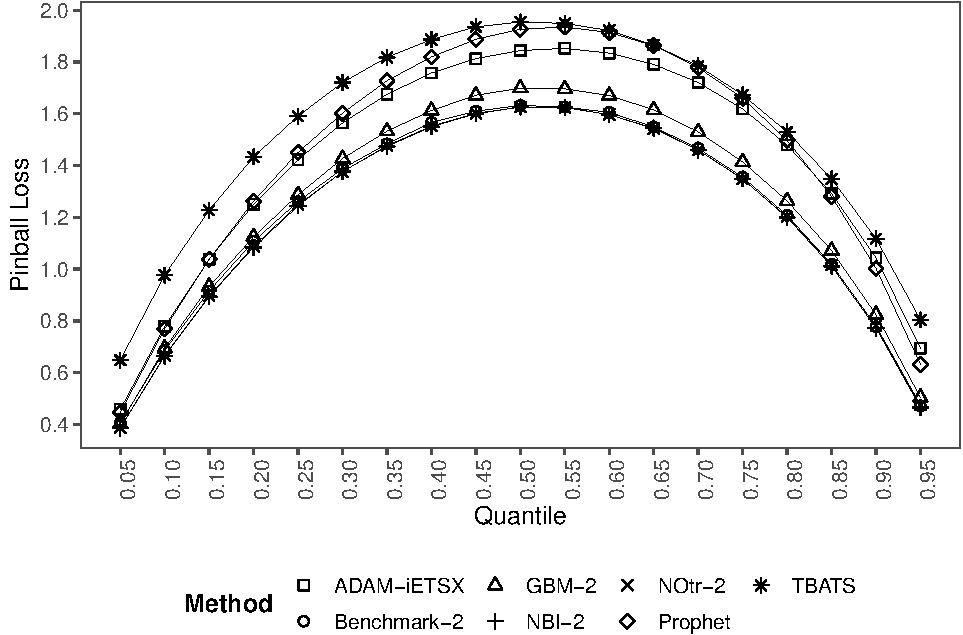
\includegraphics[width=0.9\linewidth]{paper_files/figure-latex/Pinball-1} 

}

\caption{Pinball loss values over different quantiles.}\label{fig:Pinball}
\end{figure}

\begin{figure}[H]

{\centering 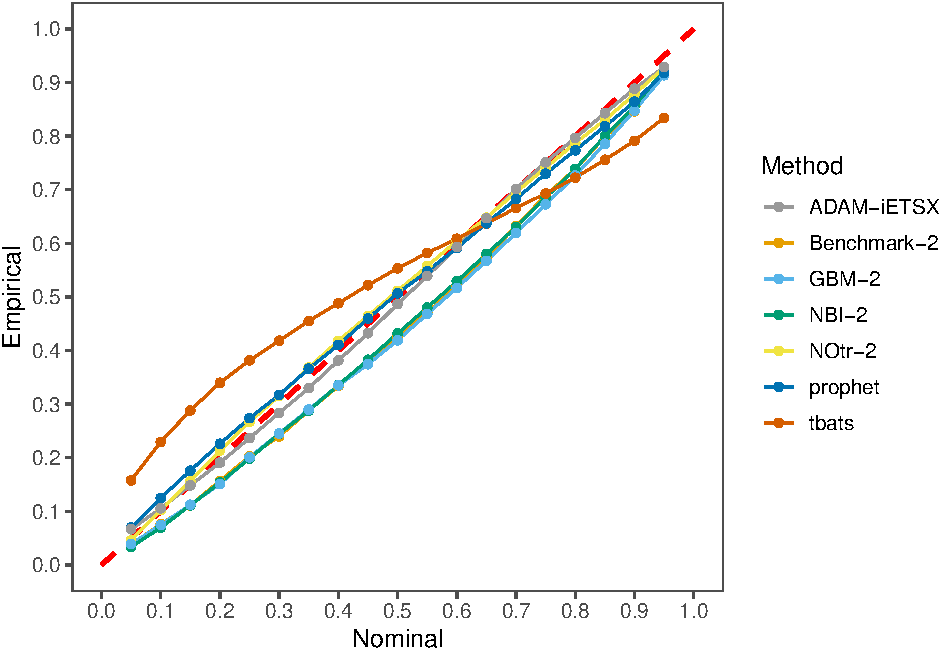
\includegraphics[width=0.9\linewidth]{paper_files/figure-latex/Reliability-1} 

}

\caption{Reliability score, showing the relation between empirical and theoretical quantiles.}\label{fig:Reliability}
\end{figure}

\begin{figure}[H]

{\centering 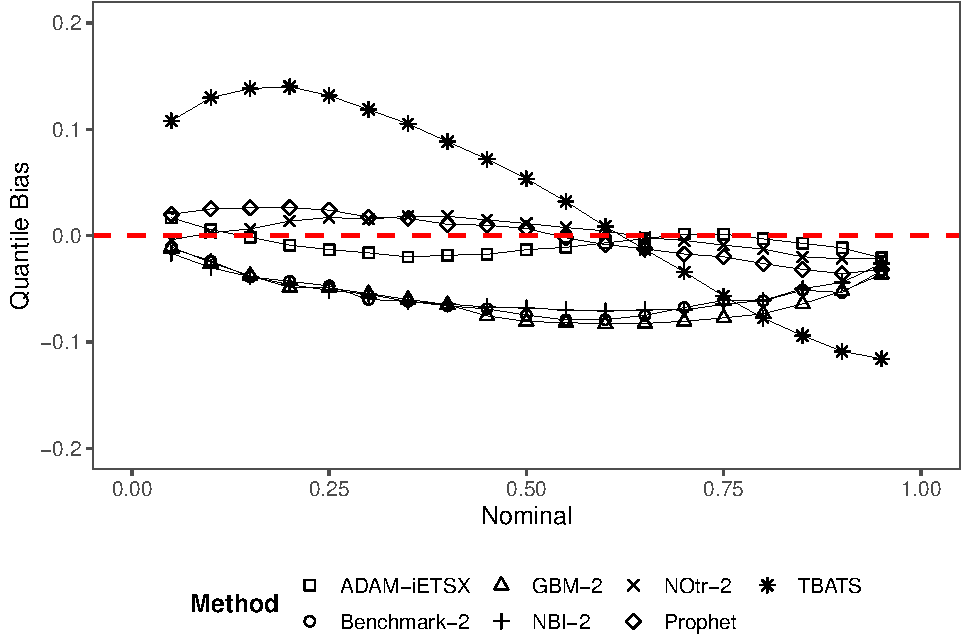
\includegraphics[width=0.9\linewidth]{paper_files/figure-latex/quantile-bias-1} 

}

\caption{Quantile bias vs the nominal quantiles.}\label{fig:quantile-bias}
\end{figure}

\begin{table}[!h]

\caption{\label{tab:tab-results}Summary of studies in hourly emergency care forecasting}
\centering
\fontsize{11}{13}\selectfont
\begin{tabular}[t]{lrrr}
\toprule
Method & Quantile Bias & Pinball & RMSE\\
\midrule
Benchmark-1 & 0.1047874 & 1.254491 & NA\\
Benchmark-2 & 0.0557392 & 1.217429 & NA\\
ETS(XXX) & 0.0194389 & 1.434862 & 0.0121247\\
GBM & 0.0600650 & 1.263135 & NA\\
NBI-2-I & 0.0540740 & 1.206238 & NA\\
NBI-2-log & 0.0375705 & 1.188041 & NA\\
NOtr-1 & 0.0098936 & 1.222584 & NA\\
NOtr-2 & 0.0118522 & 1.208556 & NA\\
Poisson-1 & 0.0372137 & 1.204936 & NA\\
Poisson-2 & 0.0373884 & 1.188107 & NA\\
Poisson-2-I & 0.0523937 & 1.222114 & NA\\
RegressionPoisson & 0.0929416 & 1.293524 & 0.8490258\\
Ttr-2 & 0.0140252 & 1.210105 & NA\\
faster & 0.1862190 & 35.051012 & NA\\
iETSCeiling & 0.0104673 & 1.419490 & NA\\
iETSXSeasonal & 0.0104673 & 1.417260 & 0.0896228\\
qreg-1 & 0.0643451 & 1.340557 & NA\\
tbats & 0.0855702 & 1.536080 & 0.4859770\\
\bottomrule
\end{tabular}
\end{table}

Evaluation metrics from the test period are presented in Table \ref{tab:tab-results}. They are ordered by Quantile Bias. The five models identified above have a Quantile Bias of 0.014 or less, which is substantially lower than the next group of forecast with Quantile Biases of 0.037 and above, ETS being the only exception with a value of 0.019.

\begin{figure}[H]

{\centering 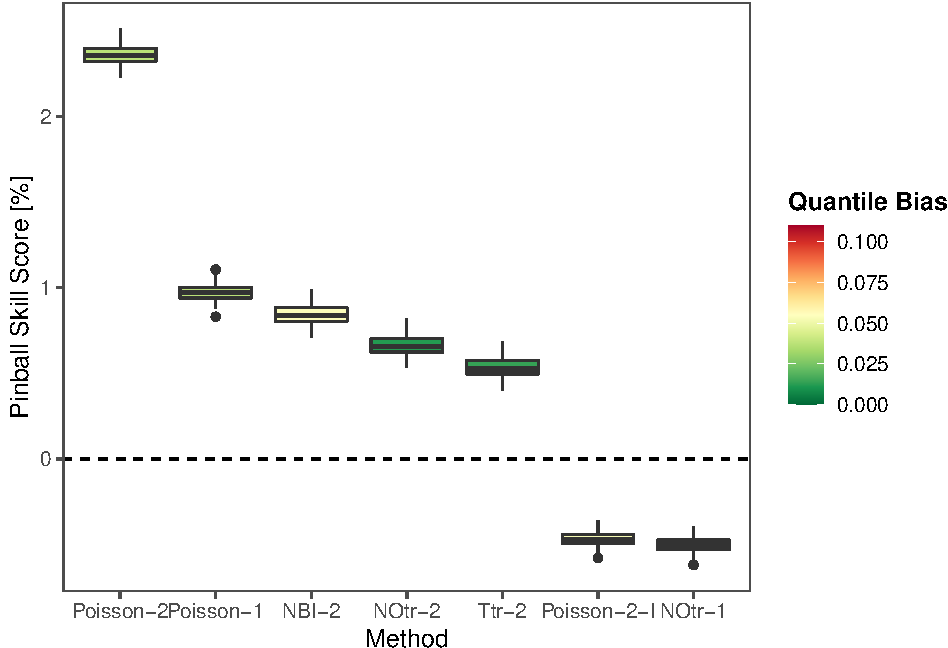
\includegraphics[width=0.7\linewidth]{paper_files/figure-latex/Skill-rel2bench-reduced-1} 

}

\caption{Skill score ...}\label{fig:Skill-rel2bench-reduced}
\end{figure}

\begin{figure}[H]

{\centering 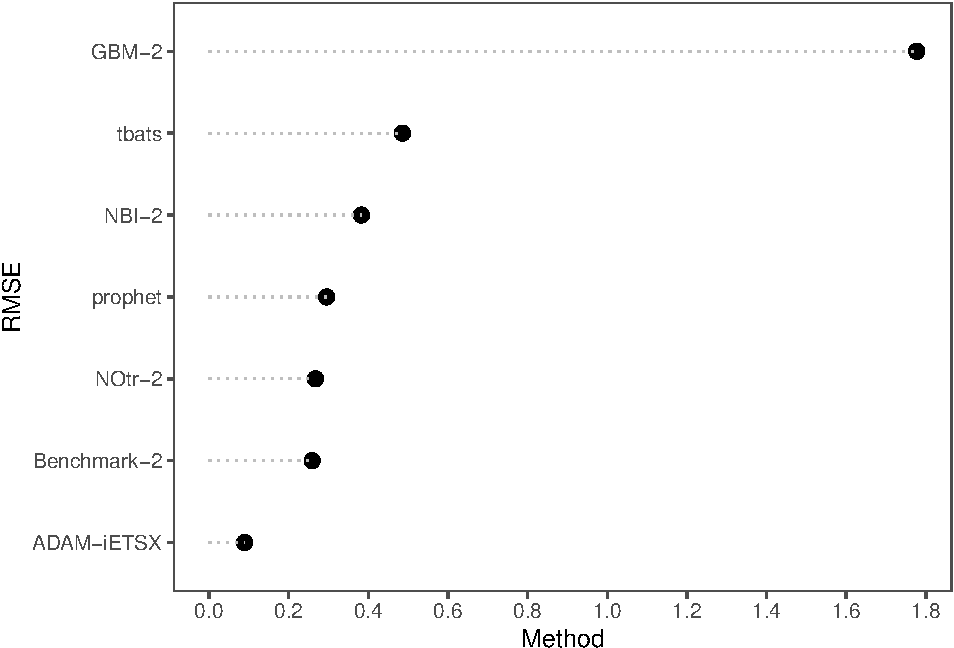
\includegraphics[width=0.7\linewidth]{paper_files/figure-latex/rmse-1} 

}

\caption{RMSE ...}\label{fig:rmse}
\end{figure}

\begin{figure}[H]

{\centering 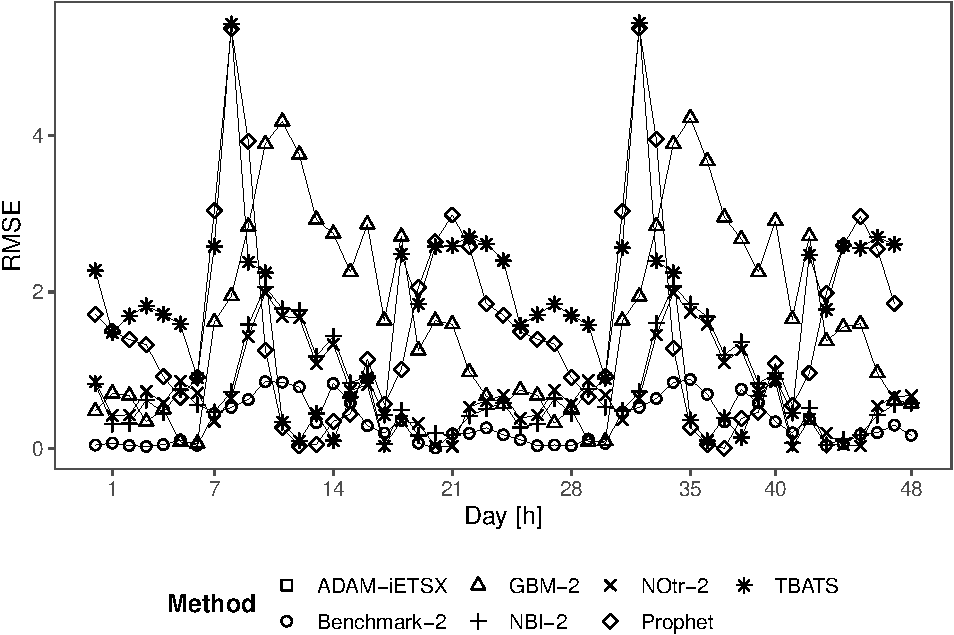
\includegraphics[width=0.7\linewidth]{paper_files/figure-latex/lead-time-rmse-1} 

}

\caption{RMSE ...}\label{fig:lead-time-rmse}
\end{figure}

\begin{figure}[H]

{\centering 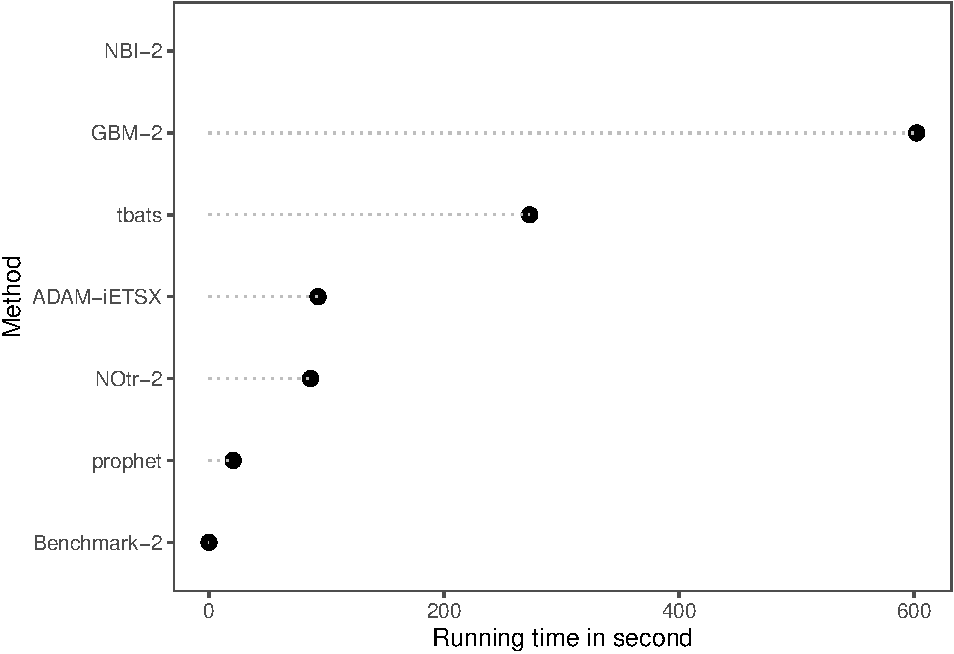
\includegraphics[width=0.7\linewidth]{paper_files/figure-latex/time-1} 

}

\caption{Running time ...}\label{fig:time}
\end{figure}

\begin{figure}[H]

{\centering 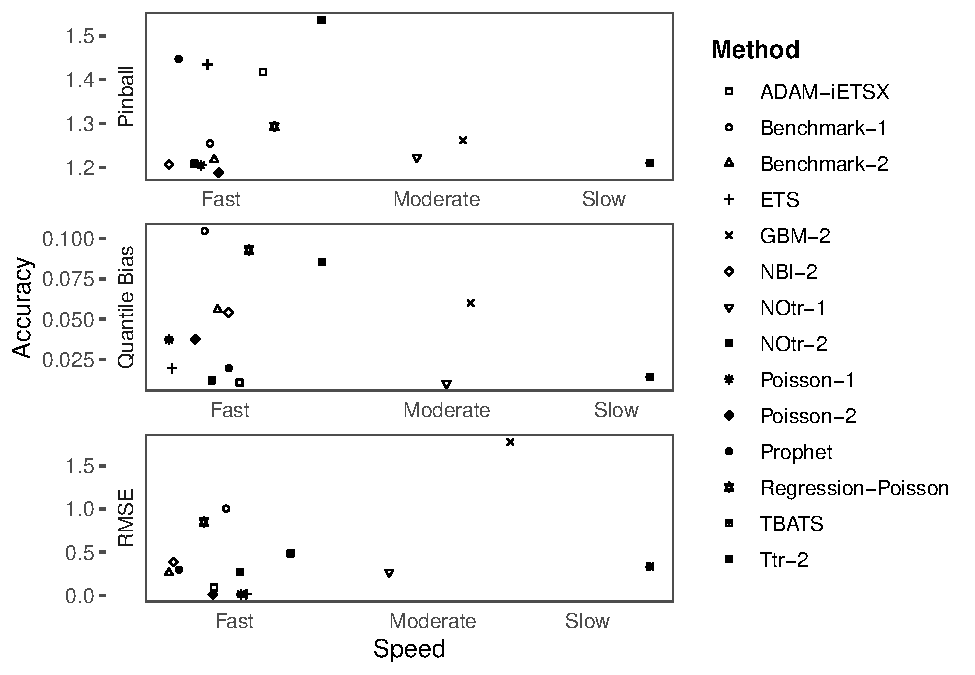
\includegraphics[width=0.7\linewidth]{paper_files/figure-latex/time-accuracy-1} 

}

\caption{Running time vs. forecast accuracy}\label{fig:time-accuracy}
\end{figure}

One more thing to notice is that the ADAM-iETSX model with rounded up quantiles did not perform better than the simpler one with continuous ones. This implies that the rounding is not necessary in general, but if integer values are needed (for example, to decide how many nurses to have), then using the continuous model and then rounding up the quantiles could be considered as a reasonable strategy.

\hypertarget{conclusion}{%
\section{Conclusion}\label{conclusion}}

\hypertarget{appendices}{%
\section{Appendices}\label{appendices}}

\hypertarget{quantiles_ceiling}{%
\subsection{Quantiles of rounded up random variables}\label{quantiles_ceiling}}

Before proceeding with the proof we need to give the definition of the quantiles of the continuous and rounded up random variables:

\begin{equation} \label{eq:quantCeil1}
    P \left(y_t < k \right) = 1 - \alpha ,
\end{equation}

and

\begin{equation} \label{eq:quantCeil2}
    P \left(\lceil y_t \rceil \leq n \right) \geq 1 - \alpha ,
\end{equation}

where \(n\) is the quantile of the distribution of rounded up values (the smallest integer number that satisfies the inequality \eqref{eq:quantCeil2}) and \(k\) is the quantile of the continuous distribution of the variable.

In order to prove that \(n = \lceil k \rceil\), we need to use the following basic property:

\begin{equation} \label{eq:quantCeil3}
    \lceil y_t \rceil \leq n \iff  y_t \leq n,
\end{equation}

which means that the rounded up value will always be less than or equal to \(n\) if and only if the original value is less than or equal to \(n\). Taking into account \eqref{eq:quantCeil3}, the probability \eqref{eq:quantCeil2} can be rewritten as:

\begin{equation} \label{eq:quantCeil4}
    P \left(y_t \leq n \right) \geq 1 - \alpha .
\end{equation}

Note also that the following is true:

\begin{equation} \label{eq:quantCeil5}
    P \left(\lceil y_t \rceil \leq n-1 \right) = P \left(y_t \leq n-1 \right) < 1 - \alpha .
\end{equation}

Taking the inequalities \eqref{eq:quantCeil1}, \eqref{eq:quantCeil2}, \eqref{eq:quantCeil4} and \eqref{eq:quantCeil5} into account, the following can be summarised:

\begin{equation} \label{eq:quantCeil6}
    P \left(y_t \leq n-1 \right) < P \left(y_t < k \right) \leq P \left(y_t \leq n \right) ,
\end{equation}

which is possible only when \(k \in (n-1, n]\), which means that \(\lceil k \rceil = n\). So the rounded up quantile of continuous random variable \(y_t\) will always be equal to the quantile of the descritised value of \(y_t\):

\begin{equation} \label{eq:ceilingAndQuantiles1}
    \left \lceil Q_\alpha(y_t) \right \rceil = Q_\alpha \left(\lceil y_t \rceil \right) .
\end{equation}

It is also worth noting that the same results can be obtained with the floor function instead of ceiling, following the same logic. So the following equation will hold for all \(y_t\) as well:
\begin{equation} \label{eq:floorAndQuantiles1}
    \left \lfloor Q_\alpha(y_t) \right \rfloor = Q_\alpha \left(\lfloor y_t \rfloor \right) .
\end{equation}

\renewcommand\refname{References}
\bibliography{mybibfile.bib}


\end{document}
